\documentclass{article}

\usepackage[paper=letterpaper,margin=2.5cm]{geometry} % Set Margins

\usepackage{placeins}

%% Math and math fonts
\usepackage{amsmath, amsthm, amssymb, amsfonts}
\usepackage{bbm} % for \mathbbm{1}

\usepackage{amsmath}

% date
\usepackage[nodayofweek]{datetime}

% Color
\usepackage{color, xcolor}

% Misc
\usepackage{environ}  % \collect@body in asmmath
\usepackage{graphicx} % \includegraphics options
\usepackage{mdframed} % text boxes
\usepackage{indentfirst} % Indent first paragraph after section header
\usepackage[shortlabels]{enumitem} % Control enumerate items with [(a)]
\usepackage{comment} % Comments
\usepackage{fancyhdr} % Headers and footers

% Tables
\usepackage{array}

% Sub-figures and figure placement
\usepackage{caption}
\usepackage{subcaption}
\usepackage{float} 

% Graphing
\usepackage{pgfplots}
\pgfplotsset{compat=1.17}
\usepackage{tikz}

% Title Placement
\usepackage{titling}
\setlength{\droptitle}{-6em}

%set indent to 
\setlength{\parindent}{0pt}

% Hyper refs
\usepackage{hyperref}
\hypersetup{
    colorlinks=true,
    linkcolor=blue,
    urlcolor  = blue,
    filecolor=magenta,      
    urlcolor=blue,
    citecolor = blue,
    anchorcolor = blue
}

% % Citation management
\usepackage{natbib}
\bibliographystyle{abbrvnat}
\setcitestyle{authordate,open={(},close={)}}

\pagestyle{fancy}

\usepackage[paper=letterpaper,margin=2.5cm]{geometry} % Set Margins

%% Math and math fonts
\usepackage{amsmath, amsthm, amssymb, amsfonts}
\usepackage{bbm} % for \mathbbm{1}

% date
\usepackage[nodayofweek]{datetime}

% Color
\usepackage{color, xcolor}

% Misc
\usepackage{environ}  % \collect@body in asmmath
\usepackage{graphicx} % \includegraphics options
\usepackage{mdframed} % text boxes
\usepackage{indentfirst} % Indent first paragraph after section header
\usepackage{comment} % Comments
\usepackage{fancyhdr} % Headers and footers

% Tables
\usepackage{array}

% Sub-figures and figure placement
\usepackage{caption}
% \usepackage{subcaption}
\usepackage{float} 

% Graphing
\usepackage{pgfplots}
\pgfplotsset{compat=1.17}
\usepackage{tikz}

% Title Placement
\usepackage{titling}
\setlength{\droptitle}{-6em}

%set indent to 
\setlength{\parindent}{0pt}

% Hyper refs
\usepackage{hyperref}
\hypersetup{
    colorlinks=true,
    linkcolor=blue,
    urlcolor  = blue,
    filecolor=magenta,      
    urlcolor=blue,
    citecolor = blue,
    anchorcolor = blue
}

% % Citation management
\usepackage{natbib}
\bibliographystyle{abbrvnat}
\setcitestyle{authordate,open={(},close={)}}

\newcolumntype{M}{>{$}c<{$}} % Define a new column type for math mode


% ----------------------------------------
% TITLE
% ----------------------------------------

\pagestyle{fancy}

\lhead{Creel}
\chead{Differential Equations}
\rhead{AMES}

\title{AMES Class Notes -- Week 11, Wednesday: Differential Equations, Cont.}
\author{Andie Creel}

\begin{document}
\maketitle

\section{Review from last week}
Consider we're at a \textbf{steady state} 
\begin{align*}
    \dot x = \frac{dx}{dt} = 0 
\end{align*}

solve for x to find the stock value that create a system where the stock doesn't change through time. (\textit{ie} a carrying capacity). \\

Jarogon note: stable equilibrium =  global/local attractor $\subseteq$ steady states = equilibrium points  = fixed points \\

Consider a population of $x$ that has a logistic growth rate. This growth rate is a second order Taylor series approximation to any arbitrary function. A second order taylor series approximation creates a "single global attractor" aka a unique stably steady state. You'll sometimes hear this called a fixed point, as well. A nice feature of second order taylor series is that they're defined over convex sets, and that guarantee's the existence of a "single global attractor" (a unique stable steady state). These are also called fixed points.\\

Returning to our logistic growth rate (which describes how the population $x$ changes through time),

\begin{align*}
    \dot x = \frac{dx}{dt} = ax( 1 - x) 
\end{align*}
The "roots" of this equation (\textit{aka} the values of $x$ that cause the growth rate to equal zero) are $x = 0$ and $x = 1$. $x = 0$ is unstable, because as soon as $x>0$ $x$ will grow away from zero. $x = 1$ is a stable equilibrium because when $x<1$, it grows towards one and when $x>1$ it shrinks towards one. \\

In conclusion, $x=0$ is an unsteady equilibrium and $x =1$ is a steady equilibrium. \\

\textbf{Finding steady states for 3rd order polynomial}

What are the levels of $x$ that produce equilibria/steady states? Which are stable and which are not?
\begin{align*}
    \dot x = \frac{dx}{dt} &= ax (\frac{x}{b} -1)(1-x)?\\
    x &= 0\\
    x &= b \\
    x &= 1
\end{align*}

Plug values just bigger and smaller than these roots into the $\dot x$ equation to see if $x$ is shrinking or growing just above or just below and equilibrium point. If the growth rate direction (\textit{ie} $x$ is shrinking or growing) pushes the population back towards the steady state population level, it's stable. \\

\begin{figure}[htp]
    \centering
    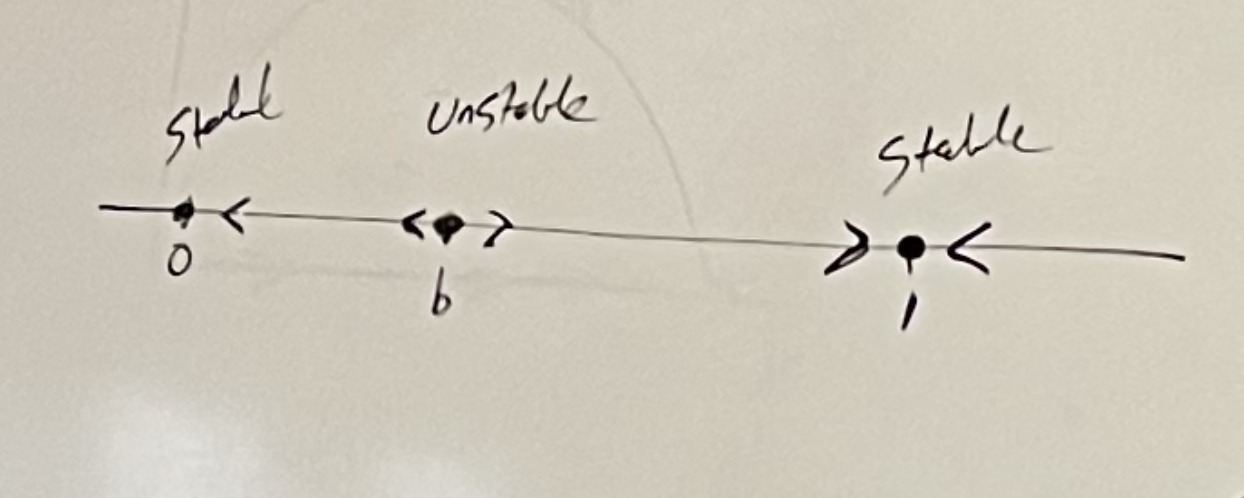
\includegraphics[width=0.5\linewidth]{Screen Shot 2023-11-15 at 11.03.06 AM.png}
    \caption{phase line}
    \label{fig:one}
\end{figure}

In this case, $x=0$ is stable, $x=b$ is unstable and $x =1$ is stable (Figure \ref{fig:one}).

\section{Lotka Voltera Model}

Consider a population of deer $x$ and a population of wolves $y$. \\

\begin{figure}[htp]
    \centering
    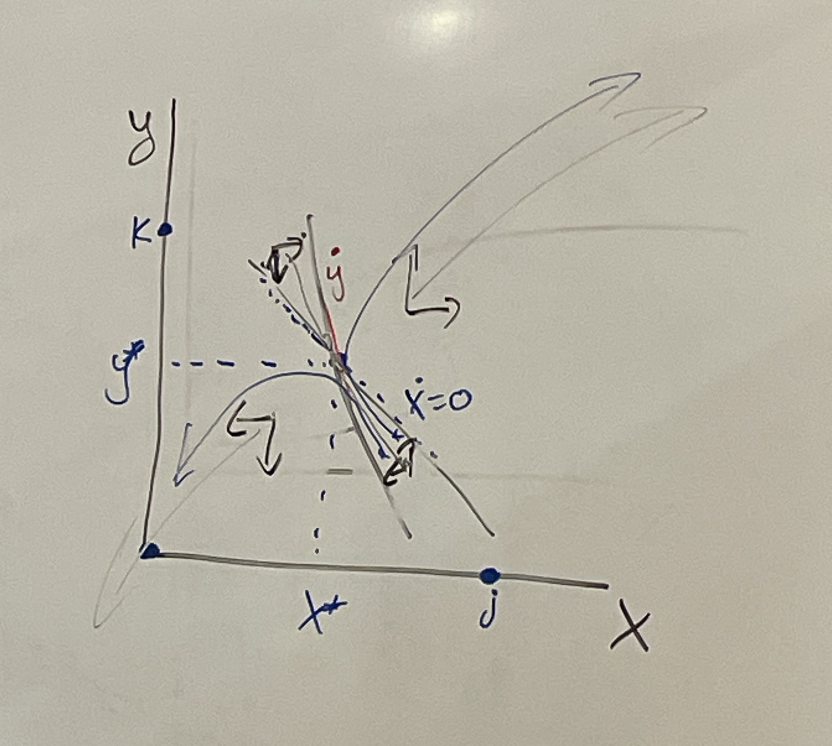
\includegraphics[width=0.5\linewidth]{Screen Shot 2023-11-15 at 11.22.55 AM.png}
    \caption{Phase plane around $(x^*, y^*)$}
    \label{fig:pset1}
\end{figure}

The growth rate of $x$ and $y$ through time are
\begin{align*}
     \dot x = \frac{dx}{dt} = ax (1 - \frac{x + \alpha y}{J}) \\
     \dot y = \frac{dy}{dt} = by (1 - \frac{\beta x + y}{K})
\end{align*}


What are the equilibrium / steady states of this system? \textit{ie} what at the pairings of $(x,y)$ that lead to $\dot x = 0$ and $\dot y = 0$. \\

From previous classes (problem set 1) we know it'll be $(0,0)$ , $(0, K)$, $(J, 0)$, $(y^*, x^*)$\\

How does the population of $y$ change with respect to the population of $x$ \textit{around an equilibrium point}? AKA what is $\frac{dy}{dx}$, \textit{around the equilibrium}? \\

Use the implicit function theorem, which considers the derivative. We are interested in when the systems (which includes two state variables, $x$ and $y$) is in a steady state. \\

Because we're interested in the dynamics around the equilibrium aka  we're staying around the equilibrium point $(x^*, y^*)$, the implicit function theorem yields: 
\begin{align}
    \frac{dy}{dx} = - \frac{\frac{d \dot x}{dx}}{\frac{d \dot x}{ d y}}
\end{align}

Notes on implicit function theorem (Section 2.2): \url{https://github.com/a5creel/AMES/blob/main/class_notes/5_weds/main.pdf}\\



Now that we have $dy/dx$ at the equilibrium $(x^*, y^*)$, we can plug in different $(x,y)$ pairs that are around the equilibrium to see if the system return to $(x^*, y^*)$ or if would it travel away. This is how you draw a phase plane, depicted in Figure \ref{fig:pset1}. 


\section{Bass and Crayfish Phase Plane}

Let $x$ be the population of crayfish. Let $y$ be the population of bass. 

\begin{align*}
    \dot x = x (1 - x - \alpha y) - \frac{\delta - yx^2}{k^2 - x^2}\\
    \dot y = ry (1 - \beta x - y) + \frac{\epsilon \delta y x^2 }{k ^2 - x^2}
\end{align*}

In a system like this, we get hysteresis. It creates this phenomenon where you get very strange tipping points, where if you go past one state of the world you cannot return to the previous state easily. See Figure \ref{fig:hyst}.\\

We can also create a phase plane for this system of crayfish and bass (Figure \ref{fig:cb_phase}). In this phase plane, points $A$ and $B$ are describes some combination of crayfish and bass populations that will be a steady state equilibrium. Point $C$ would be steady IF you approached it on the dashed line. The probability of being on that approach path is functionally zero, so it is largely considered unstable. 

\begin{figure}[htp]
    \centering
    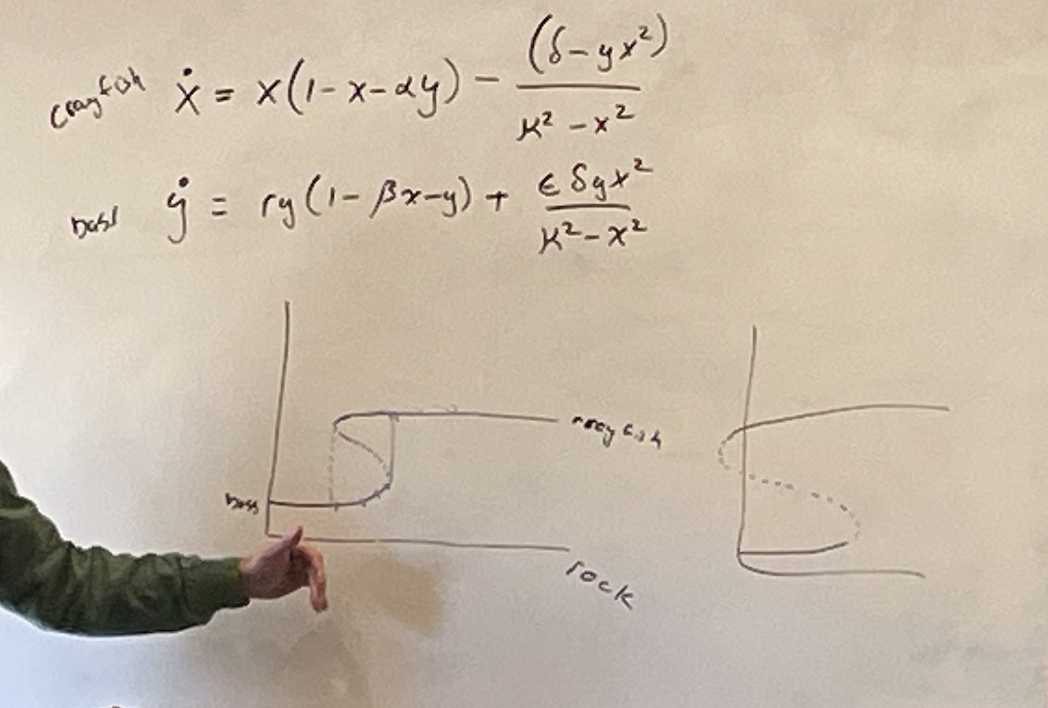
\includegraphics[width=0.7\linewidth]{hystor.png}
    \caption{crayfish population through time}
    \label{fig:hyst}
\end{figure}

\begin{figure}[htp]
    \centering
    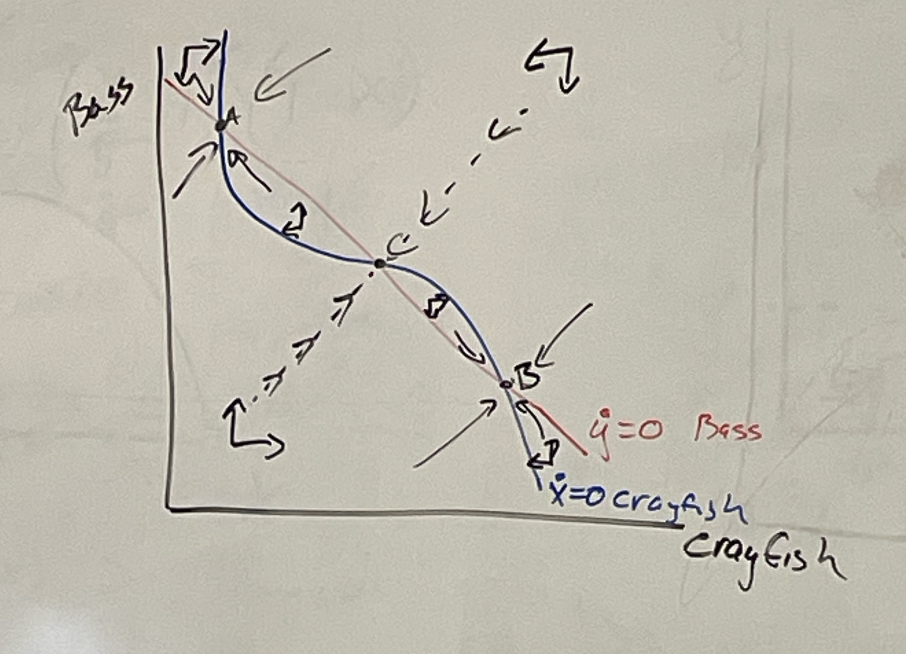
\includegraphics[width=0.5\linewidth]{Screen Shot 2023-11-15 at 11.36.44 AM.png}
    \caption{Phase plane for crayfish and bass}
    \label{fig:cb_phase}
\end{figure}

\section{Introduction to Eigen values and vectors}
Eigen values and vectors can help describe the dynamics of a system using vectors and matrices. 

Consider a system that has a linear growth rate (which we discussed last class), 
\begin{align}
    N(\tau + \epsilon) = N(\tau) e^{\lambda\epsilon}
\end{align}

\textit{I lost the thread on this example}


\subsection{Now consider a system with two state variables, x and y}

The growth rates of each state variables are 
\begin{align}
    \dot x = -0.1 x + y \\
    \dot y = \frac{100}{x^2} x + 0.1 y
\end{align}

This system can be rewritten using matrices. 

\begin{align}
    \begin{bmatrix}
        \dot x \\
        \dot y
    \end{bmatrix} = 
    \begin{bmatrix}
        -0.1 & 1 \\
        \frac{-100}{x^2} & 0.1
    \end{bmatrix}
    \begin{bmatrix}
        x \\
        y
    \end{bmatrix}
\end{align}

Next class, we will see how to use these matrices to find the eigen values and vectors, and how they describe 

\FloatBarrier

\section{Different types of equilibrium in phase planes}

There are stable, unstable, and conditionally stable equilibrium. There are different ways we can approach an equilibrium, like a spiral or a line. Sometimes, we have orbits aka stable limit cycles. \\

\begin{figure}[htp]
    \centering
    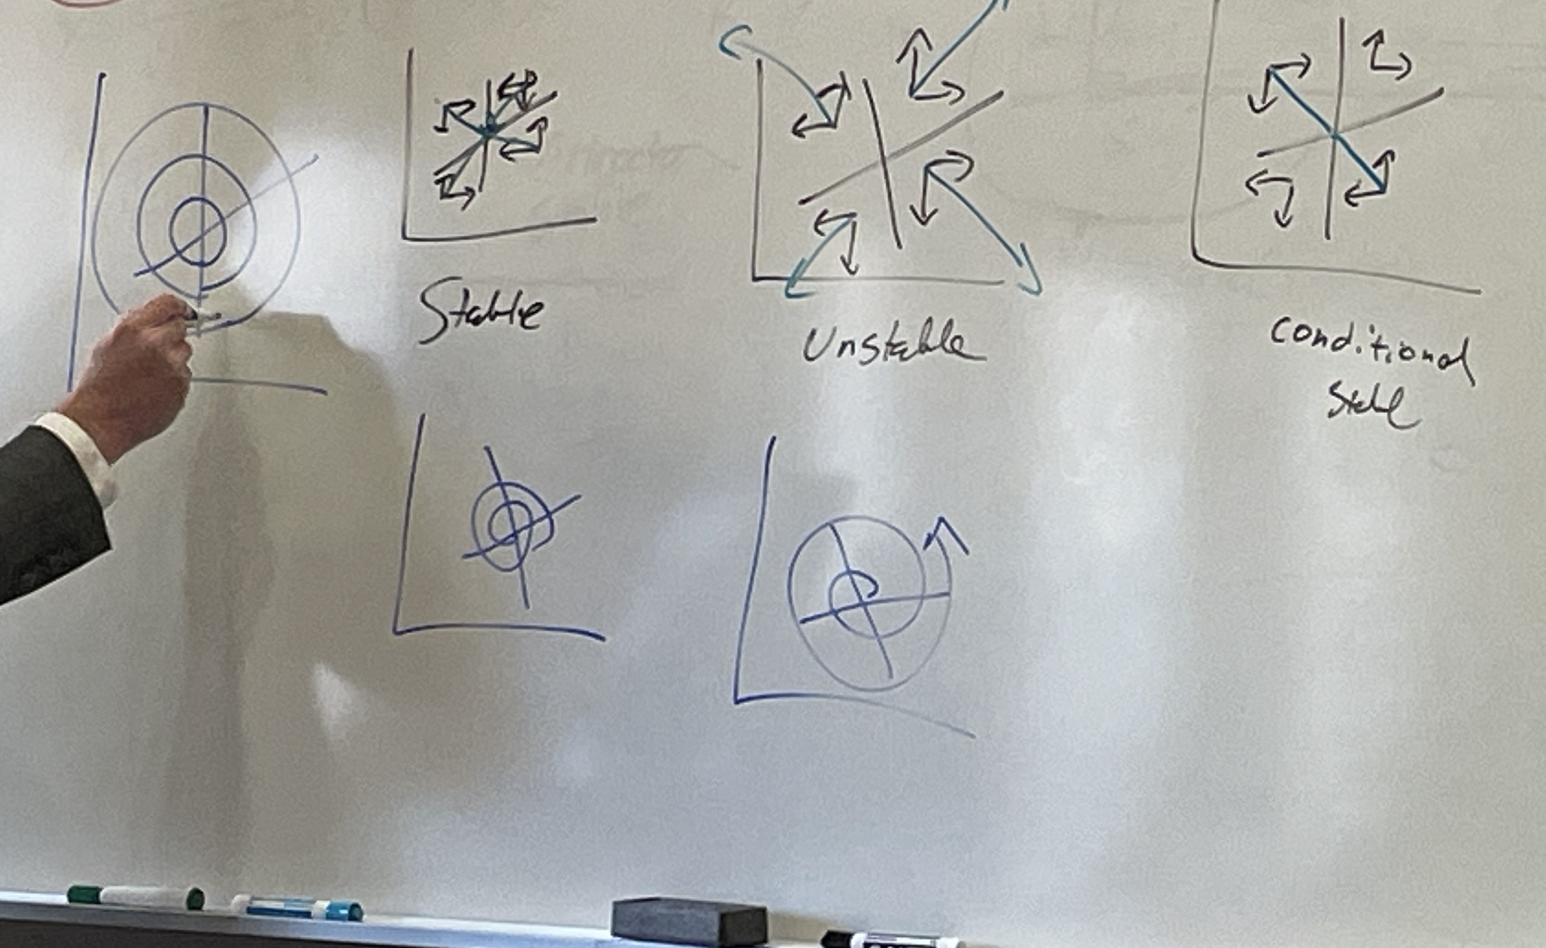
\includegraphics[width=0.5\linewidth]{Screen Shot 2023-11-15 at 11.38.59 AM.png}
    \caption{Types of equilibria}
    \label{fig:enter-label}
\end{figure}

This is all really confusing! We're going to use eigen values and eigen vectors to determine what type of equilibrium a steady state is, and what the approach path to that steady state looks like (spiral vs line). 


\section{Tipping points}

Tipping points can only be modeled with non convex sets. HOWEVER, we will not work with non-convex state spaces if we're using \textit{linear} models and most \textit{quadratic} models. Linear models and quadratic models are great approximations (shout out, taylor). HOWEVER, they will never produce scenarios with tipping points. And so, \textbf{we need to expand out standard statistical techniques to models with higher order terms to model scenarios with tipping points}. 


\end{document}